\chapter{基于子树划分的抽象语法树表征学习}
\label{chap:AST}
本章主要对本文提出的基于子树划分的抽象语法树表征学习方法进行详细介绍,首先介绍其研究动机,其次阐述其具体方法设计与实现,最后进行实验验证。

\section{研究动机}
\label{sec:ASTMotivation}
基于Token的代码表征通常将代码视为自然语言文本,根据程序员的开发风格不同,代码的命名方式、上下文组织方式也不一样,因此在代码表征过程中通常会产生很多噪声,并且遗漏源代码的结构信息。为了提高代码表征能力,研究人员提出了基于抽象语法树的代码表征方法。抽象语法树是源代码语法结构的一种抽象表现形式,以操作数、操作符以及属性节点作为树节点,以树的形式包含了源代码中的语法信息和语法结构。基于树的方法利用了树本身的结构化特征,利用深度神经网络对树进行建模得到其向量表示,根据该特征向量完成下游代码任务,在一定程度上可以消除源代码本身的噪声,有效地提取程序的结构信息。

基于树的代码表征方法存在两种主要限制:

(1) 在使用神经网络对抽象语法树建模的过程中,梯度是通过树型拓扑结构的反向传播来计算的。由于源程序结构的复杂性,因此抽象语法树通常规模过大、节点很深,此时会出现\textbf{梯度消失}问题。具体地,在反向传播过程中,神经网络根据设定好的损失函数指导权重值的更新优化。而梯度(即损失函数对模型参数的导数)经过多层网络传递时,如果激活函数的导数接近于0,参数更新就会变得不稳定,导致模型发散或者训练不收敛,影响神经网络模型的训练效率和稳定性。

(2)由于抽象语法树的大小和深度对神经网络性能有显著影响,因此现有的基于树的方法通常将抽象语法树转化为二叉树,通过将父节点的第三个或者更多子节点移动到新的子树中进行简化。然而,在转换的过程中会改变源代码原有的语义,从而难以捕捉远程依赖关系,甚至丢失一些上下文信息。有研究发现\ref{Allamanis2017LearningTR},在抽象语法树中,具有高度关联的两个节点可能相距甚远,例如:函数调用的形参节点与实参节点存在数据依赖关系,但两者可能在转化过程中划分到不同的子树中,降低对程序的结构语法捕获能力。因此,由于转化会增加抽象语法树高度,从而加重了梯度消失问题,削弱神经模型捕捉更真实和复杂语义的能力。

因此,针对梯度消失问题,本文提出了一种基于子树划分的抽象语法树表征方法,该方法将大型抽象语法树分割为小型语句树序列,在减小抽象语法树大小和深度的同时,通过捕获语句树的

\section{AST表征方法设计}
\label{sec:AST}
本节将介绍基于子树划分的抽象语法树表征学习方法的详细设计,首先介绍该方法的整体框架,并从子树划分、抽象语法树表征学习两方面介绍具体设计。 

\subsection{框架概述}
\label{subsec:ASTOverview}
本文提出的基于子树划分的抽象语法树表征学习方法整体框架如图\ref{fig:astframework}所示。该框架的输入是代码片段对应的抽象语法树,输出是对应的结构特征向量,主要包括子树划分、树表征两个阶段。

\begin{figure}[H]
  \centering
  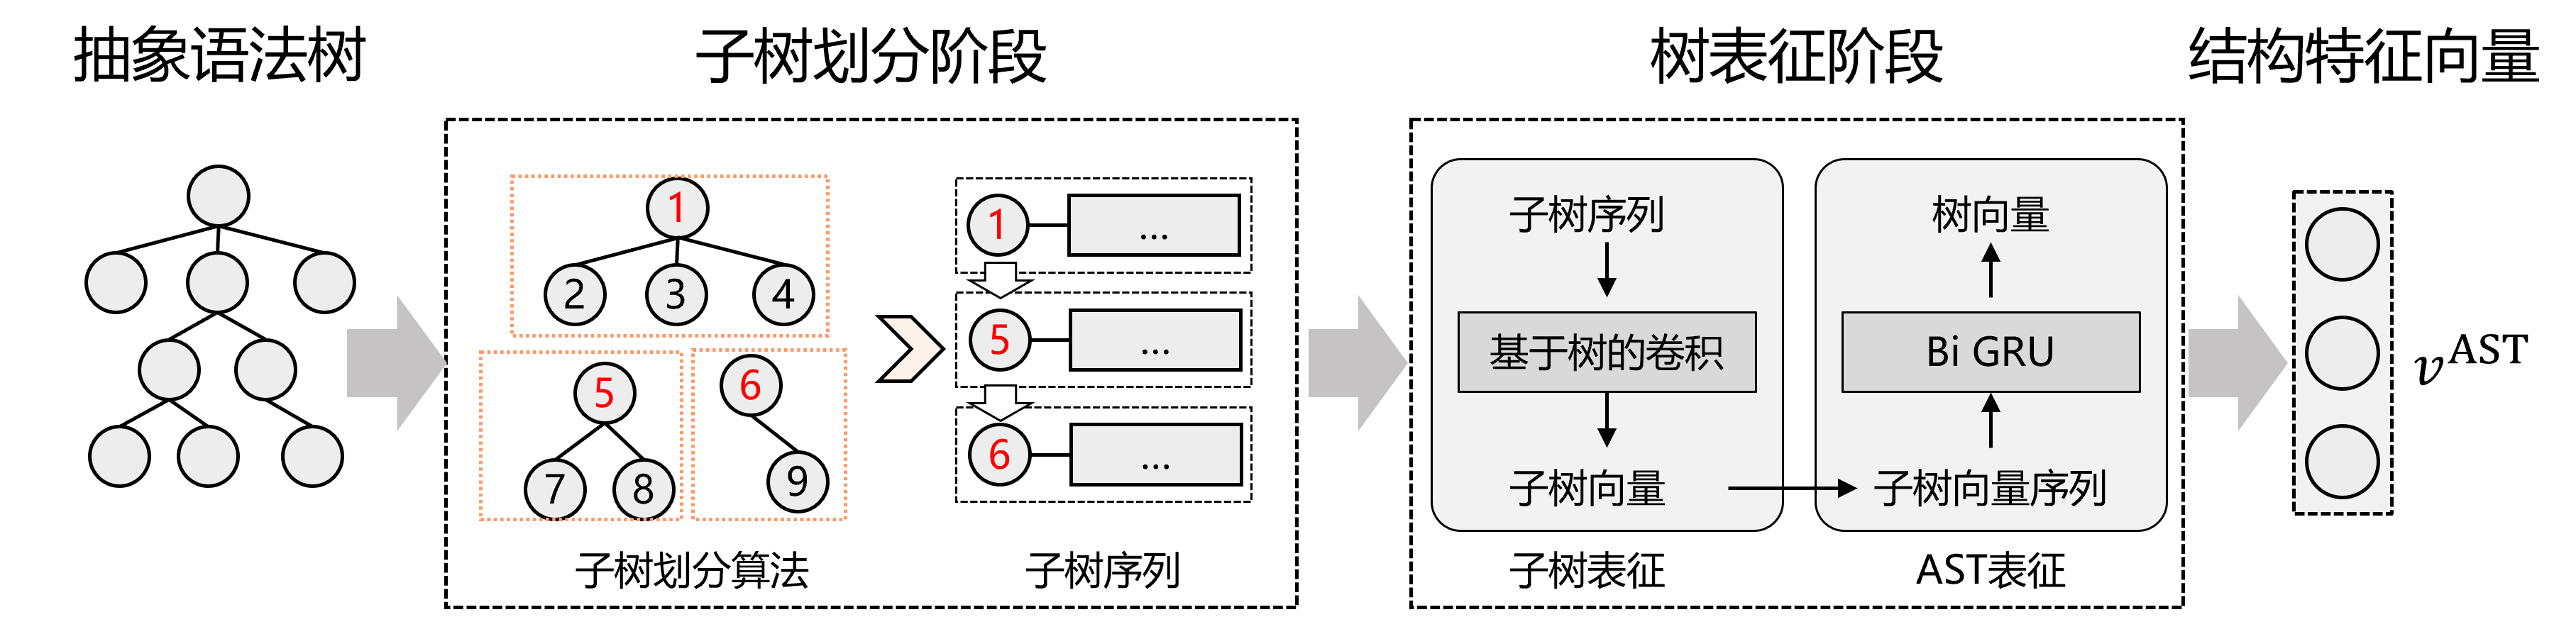
\includegraphics[width=0.95\textwidth]{figures/astframework.png}
  \caption{基于子树划分的抽象语法树表征学习框架}\label{fig:astframework}
\end{figure}

首先,子树划分阶段

其次,树表征阶段

在上述框架中,本文的创新点主要体现在子树划分阶段的子树划分算法、树表征阶段的树卷积模型设计两方面,下面将围绕这两个创新点来阐述本文的方法。

\subsection{子树划分}
\label{subsec:ASTPreModel}
针对上述问题,本文将每个大型的AST分割成小语句树序列,并通过捕获语句的词法和句法知识将每一个语句树都编码成一个向量。

\begin{algorithm}[ht]  
	\renewcommand{\algorithmicrequire}{\textbf{Input:}}
	\renewcommand{\algorithmicensure}{\textbf{Output:}}
	\caption{Subtree partitioning algorithm \(split_AST\)}  
	\label{alg2}
	\begin{algorithmic}[1]
    \Require Root node of abstract syntax tree $Root_Node$
    \Require Node set $S$
		\Ensure SubTree set $SubTrees$
    \State SubTrees = \left\{\right\}   \Comment{step1:初始化}
    \State SubTrees.append\(Root_Node\)

		\For{child_node in Root_Node.children}
      \If {child_node $\in$ S}
        SubTrees.append\(child_node\)
      \Else
        \For{subtree in SubTrees}
          \If {child_node $\in$ SubTrees.descendant}
            SubTrees.append\(child_node\)
          Else
            split_AST(subtree)
            \EndIf
        \EndFor
      \EndIf
    \EndFor \\
    \Return $SubTrees$
	\end{algorithmic}
\end{algorithm}

\subsection{抽象语法树表征学习}
\label{subsec:ASTModel}
(1)结构设计

在得到一个语句向量序列后,将语句向量序列输入Tree LSTM网络中生成代码片段的结构向量表示。与标准LSTM结构类似,Tree-LSTM神经网络中每个神经元都包括类似的输入门,输出门和隐层输出。不同的是Tree-LSTM单元中门向量和神经元状态的更新依赖于所有与之相关的子单元的状态,另外,Tree-LSTM拥有多个遗忘门,分别对应当前节点的每个子节点,因此 Tree-LSTM可以选择性地从子节点中获取信息,从而保存语义信息更加丰富的子节点的信息。通过Tree LSTM模型,本文能够学习到基于抽象语法树的结构向量,通过这种连续向量表现基于树的理解认知层次,获取程序的结构信息,创建更高抽象层次上的表示,从而提高后续代码克隆检测任务的精度。



为了提高抽象语法树维度代码表征能力,本文选取树卷积网络对上述得到子树序列进行建模,使用双向门控循环单元(BiGRU)对整个树进行建模。具体的模型设计如图\ref{fig:astmodel}所示。该模型主要包括子树卷积层、双向门控循环层(BiGRU)、自注意力机制层(Attention)、输出层。
\begin{figure}[H]
  \centering
  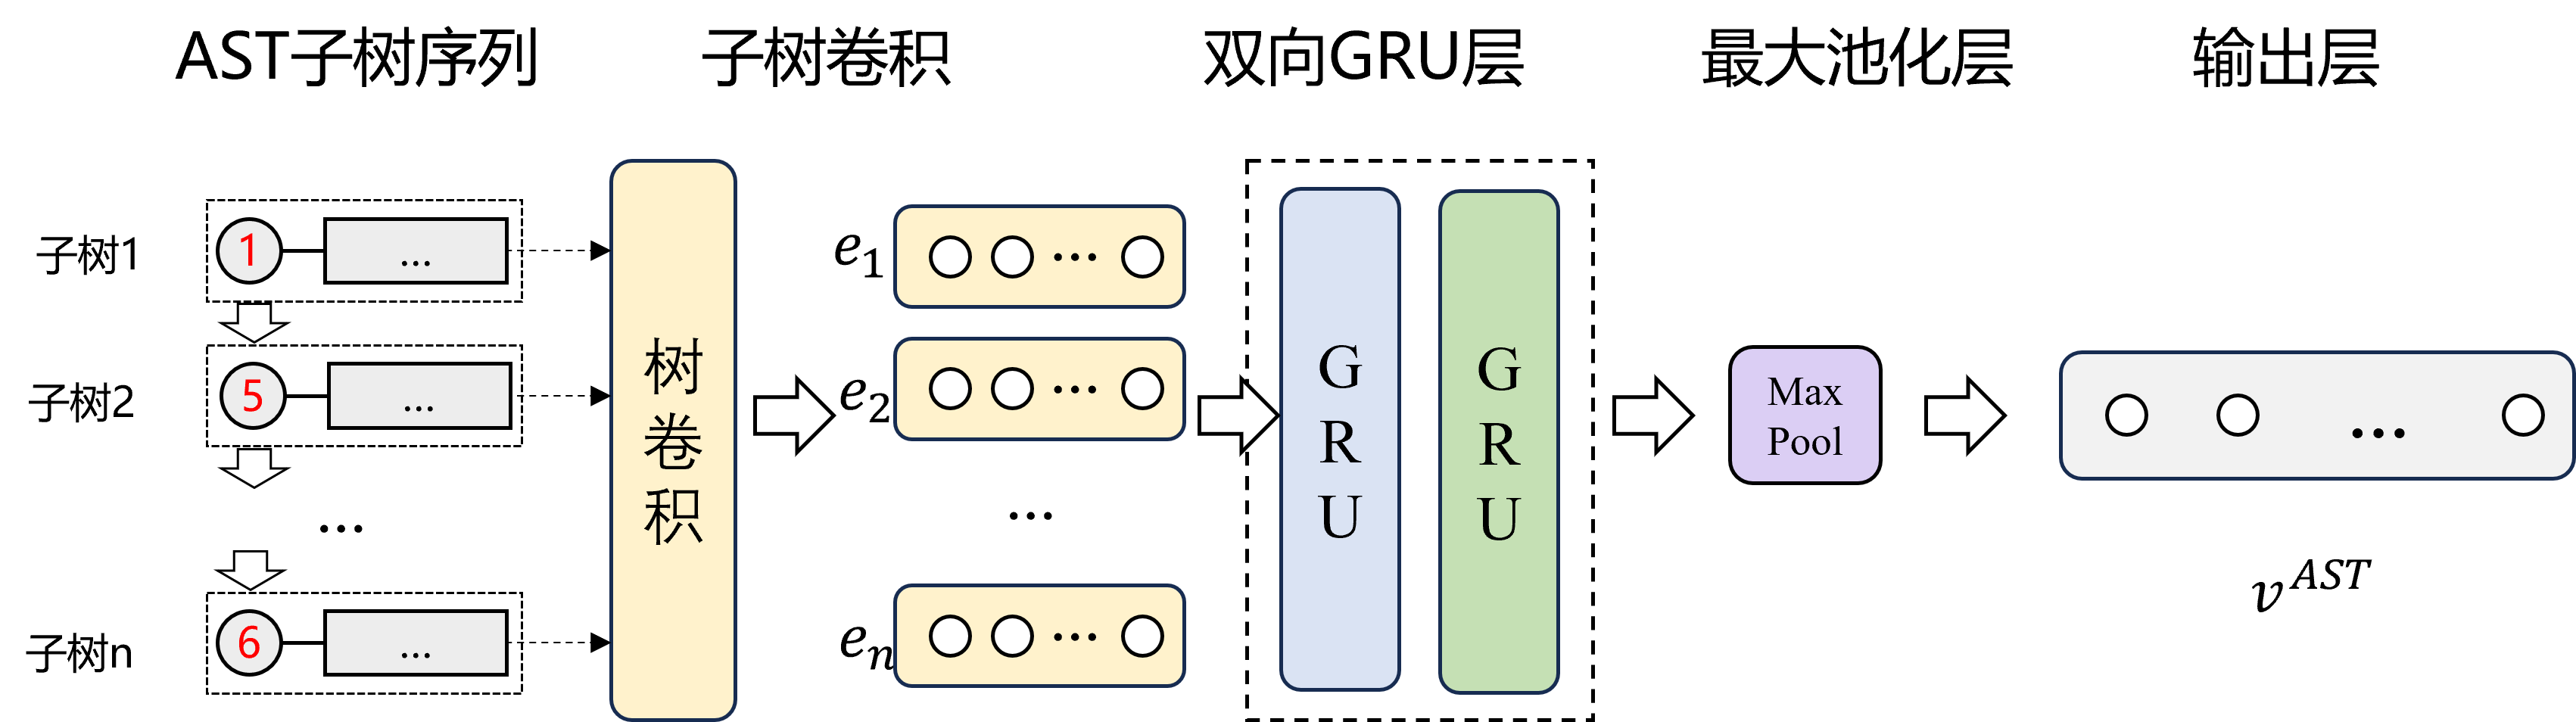
\includegraphics[width=0.85\textwidth]{figures/astmodel.png}
  \caption{抽象语法树表征模型设计}\label{fig:astmodel}
\end{figure}

\ding{172}输入层:输入层用于向模型输入训练数据,在本方法中模型的输入为经过预训练辅助嵌入模型得到的Token序列词向量,即每个词向量对应一个输入神经元。\ding{173}双向长短时记忆层:由两层LSTM构成,同时捕获序列的双向语义信息。\ding{174}自注意力机制层:本层的主要目的是总结序列的输入特征,并将每个代码片段缩减为一个单一的密集向量。\ding{175}输出层:每个Token序列对应一个输出。

(2) 模型选型

基于树的卷积网络模型如下图\ref{fig:TreeBaseConvolution}所示。

\begin{figure}[H]
  \centering
  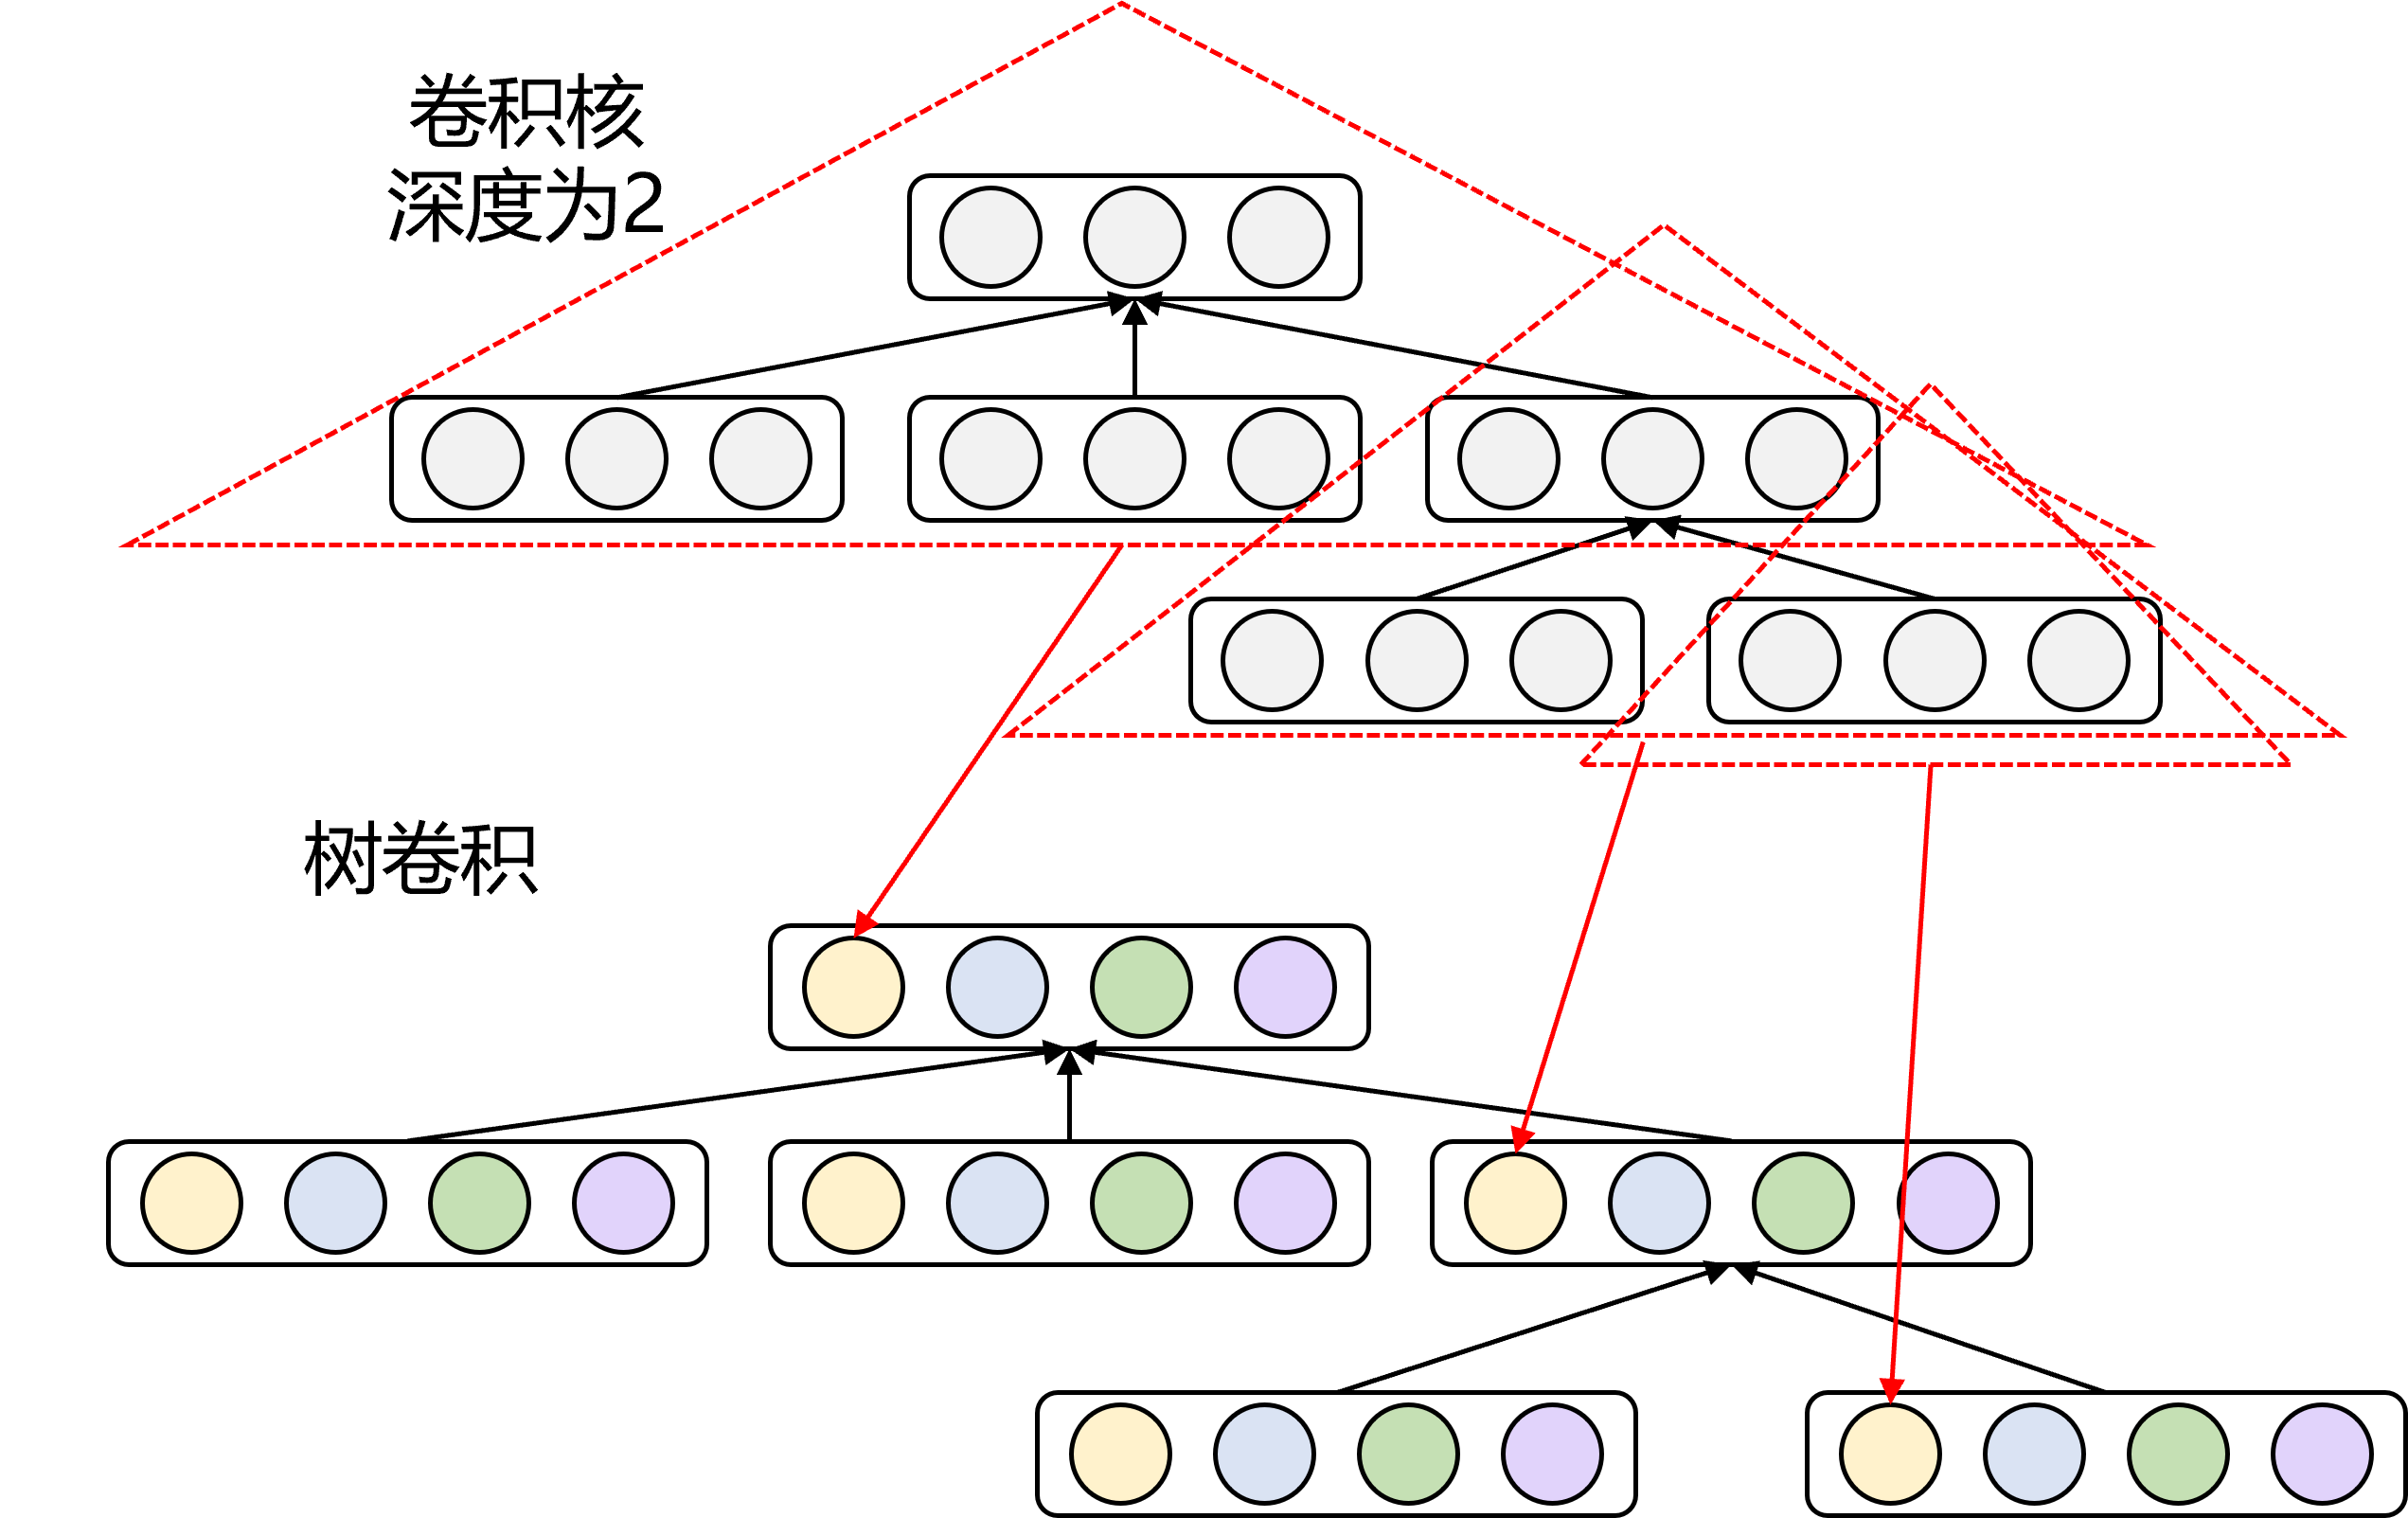
\includegraphics[width=0.85\textwidth]{figures/TreeBaseConvolution.png}
  \caption{子树表征:树卷积模型设计}\label{fig:TreeBaseConvolution}
\end{figure}


连续二叉树概念,如下图\ref{fig:Continuous}所示。

\begin{figure}[H]
  \centering
  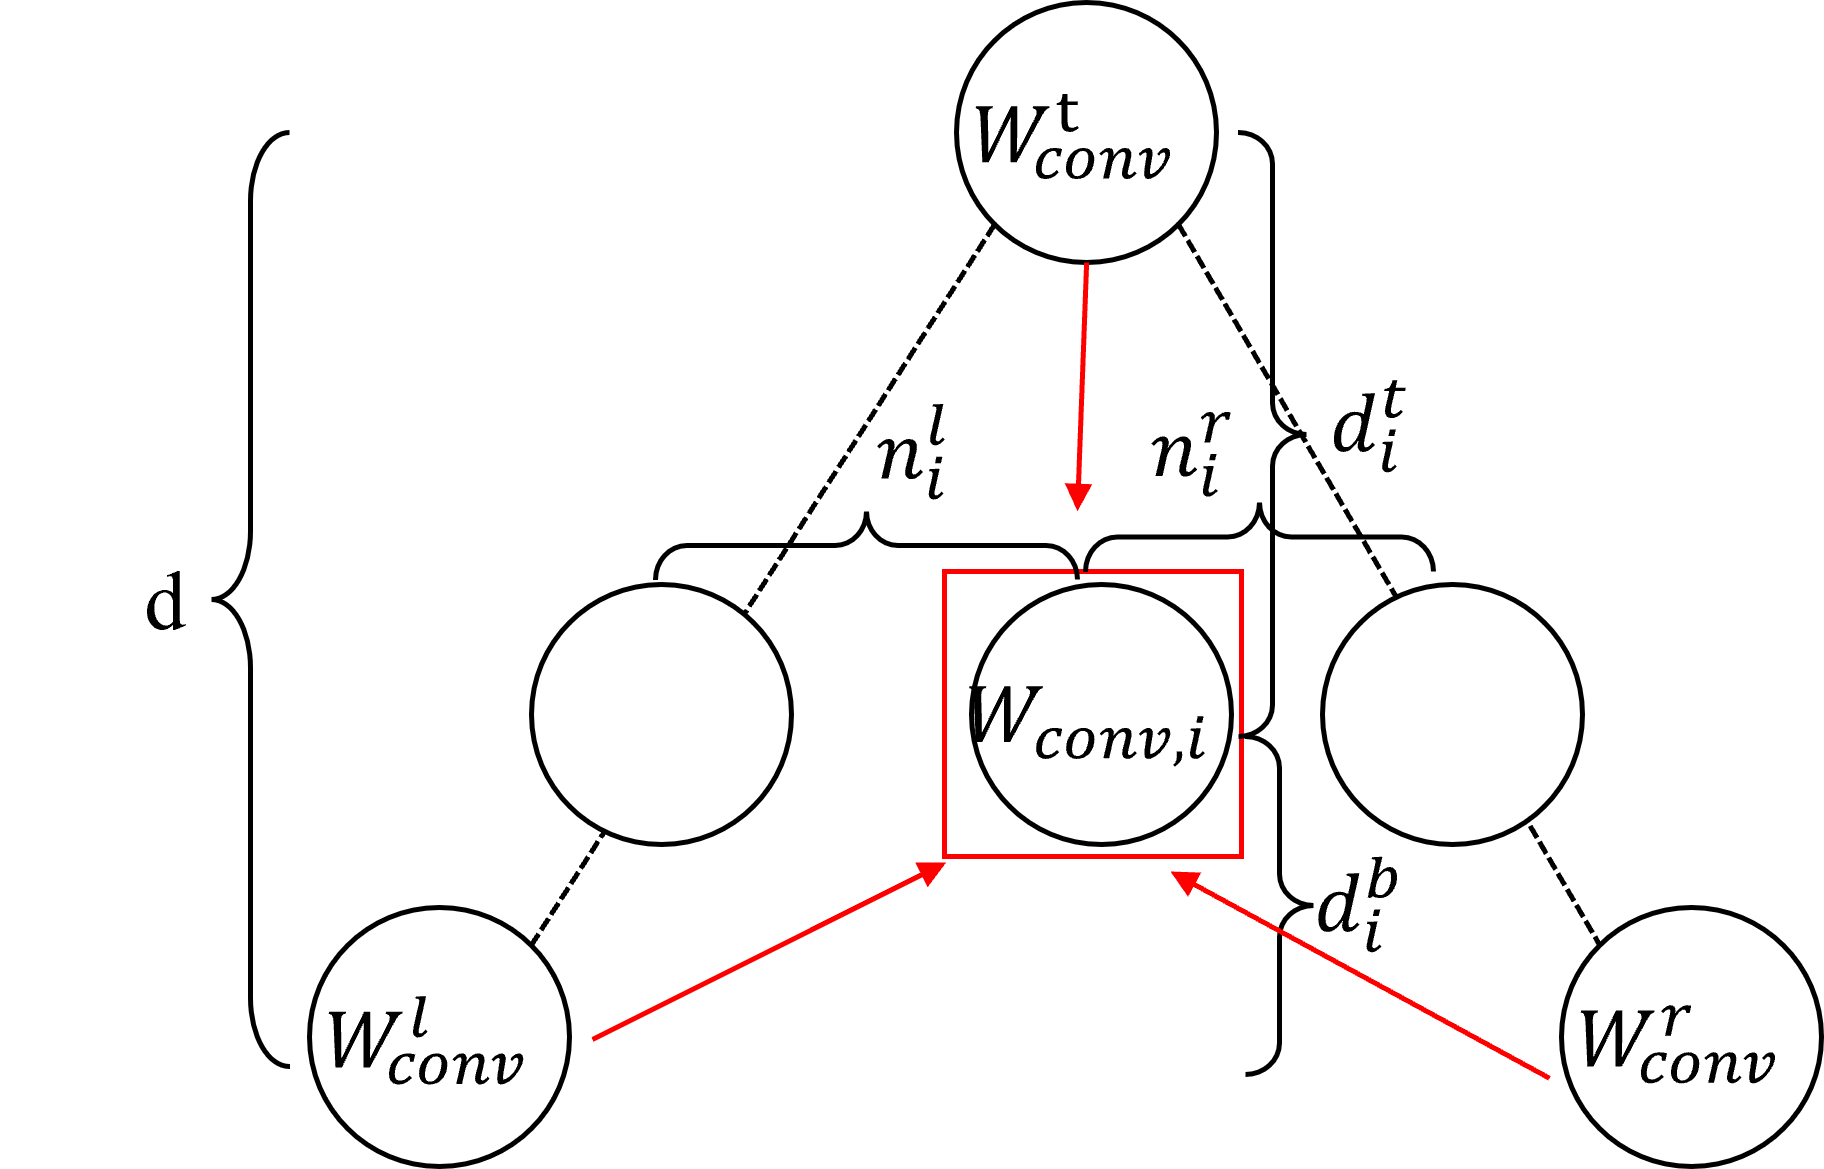
\includegraphics[width=0.85\textwidth]{figures/Continuous Binary Tree.png}
  \caption{连续二叉树}\label{fig:Continuous}
\end{figure}

\begin{equation}\label{e4.1}
  \begin{split}
    W_{\text {conv }, i}=\frac{d_{i}^{b}}{d_{i}^{b}+d_{i}^{t}} W_{\text {conv }}^{t}+\frac{d_{i}^{t}}{d_{i}^{b}+d_{i}^{t}} W_{\text {conv }, i}^{b}
  \end{split}
\end{equation}

\begin{equation}\label{e4.2}
  \begin{split}
    \begin{array}{l}
      W_{\text {conv }, i}^{b}= 
      \left\{\begin{array}{ll}
      \frac{n_{i}^{r}}{n_{i}^{r}+n_{i}^{l}} W_{\text {conv }}^{l}+\frac{n_{i}^{l}}{n_{i}^{r}+n_{i}^{l}} W_{\text {conv }}^{r} & n_{i}^{l} \geq 1 \text { or } n_{i}^{r} \geq 1, \\
      \frac{1}{2} W_{\text {conv }}^{l}+\frac{1}{2} W_{\text {conv }}^{r} & n_{i}^{l}=n_{i}^{r}=0 .
      \end{array}\right.
      \end{array}
  \end{split}
\end{equation}


双向GRU的模型如下图\ref{fig:BiGRU}所示。
\begin{figure}[H]
  \centering
  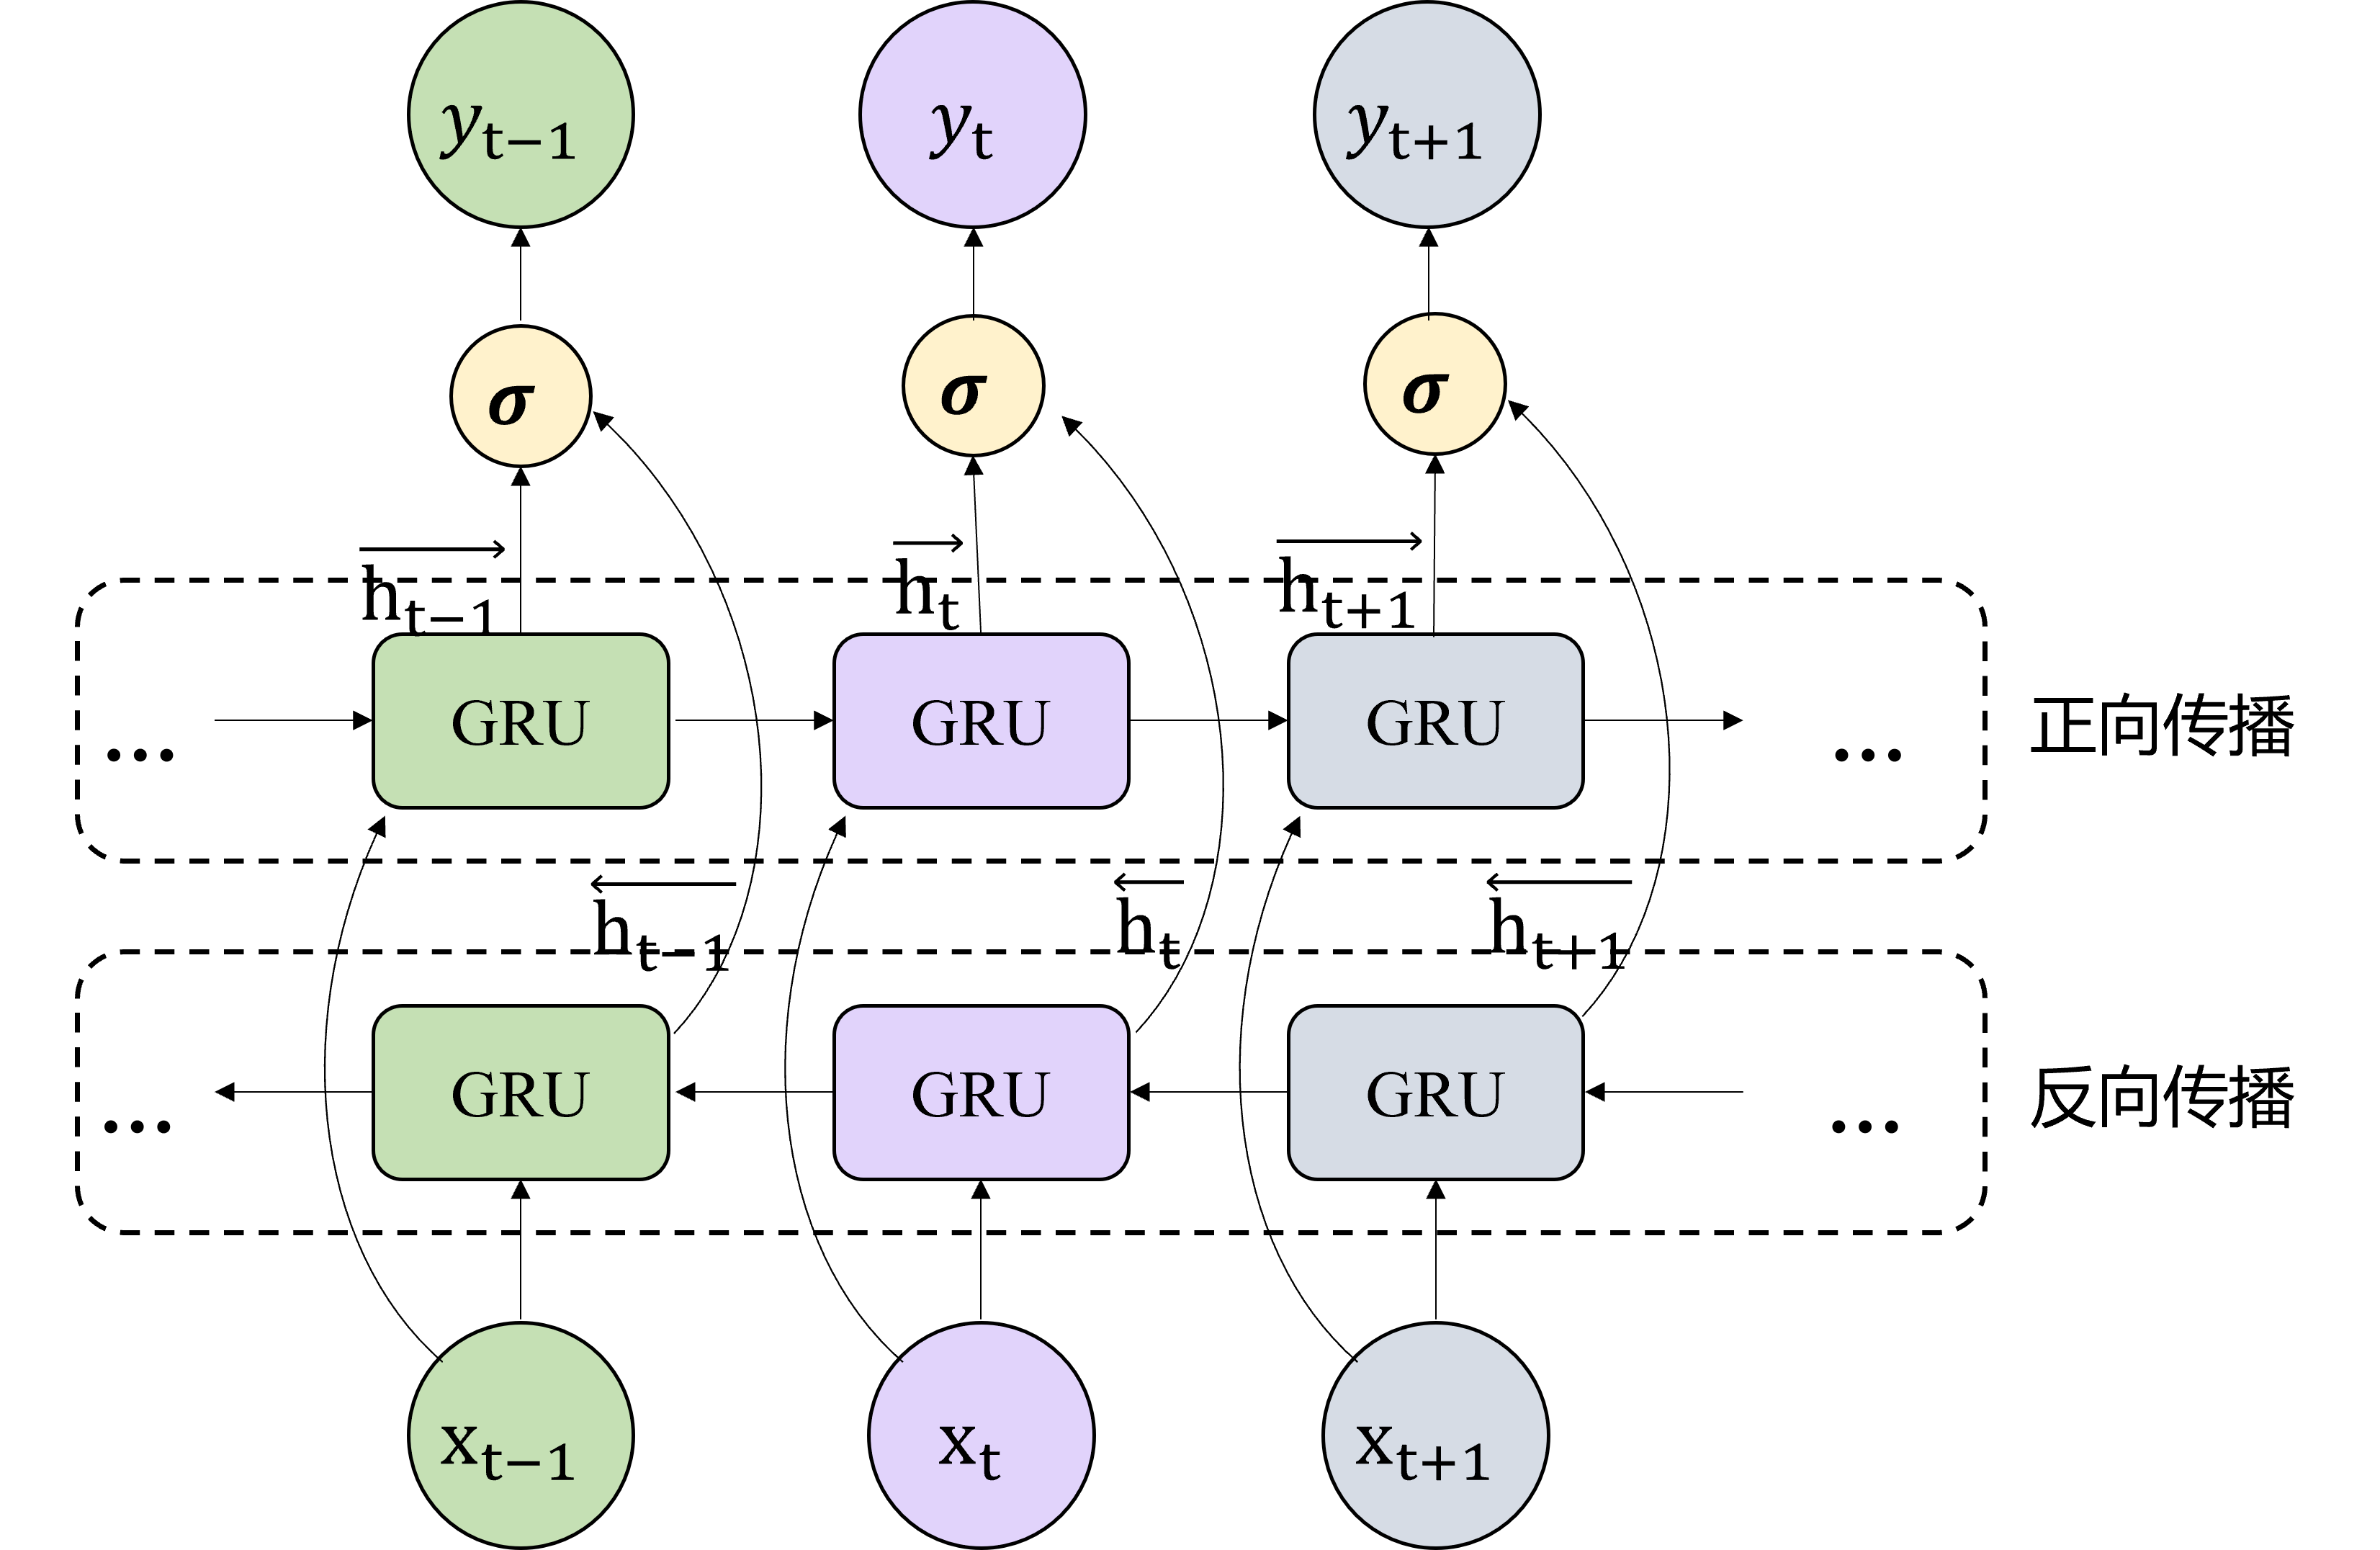
\includegraphics[width=0.85\textwidth]{figures/BiGRU.png}
  \caption{树表征:AttBiGRU模型设计}\label{fig:BiGRU}
\end{figure}

\section{AST表征方法具体实现}
\label{sec:ASTachieve}
在介绍具体实现之前,本节首先给出AST表征方法的输入:经过\ref{subsec:Preprocess}小节的代码预处理阶段,得到示例代码片段\ref{fig:code}对应的抽象语法树,如图\ref{fig:astcode}所示。仔细分析可以看出代码片段\ref{fig:ast1}对应的抽象语法树在FOR循环内部一共有13个子节点,子树高度为4;代码片段\ref{fig:ast2}对应的抽象语法树在WHILE循环内部也包含13个子节点,子树的高读为4,两者子节点个数相同;而代码片段\ref{fig:ast3}对应的抽象语法树在FOR循环中共有18个子节点,子树高度为6,与代码片段\ref{fig:ast1}对应的抽象语法树在根节点的下一层、下两层中1-9号节点架构相似。
\begin{figure}[htbp]
  \centering  %居中
  \subfigure[代码片段1对应的AST]{   %第一张子图
      \centering    %子图居中
      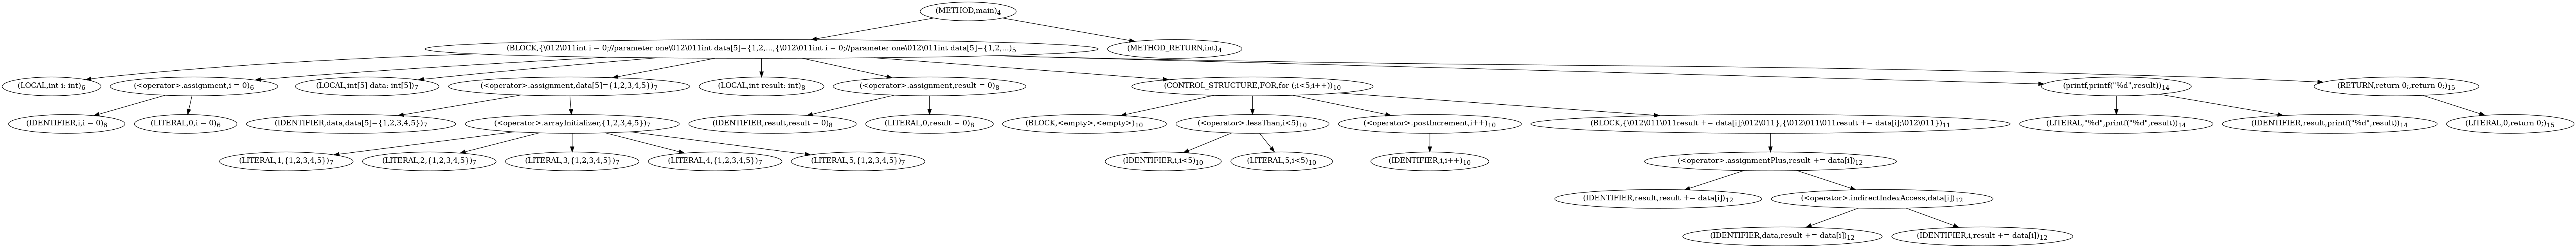
\includegraphics[width=0.3\textwidth]{figures/ast1}  
      \label{fig:ast1} %引用标签
  }
  \subfigure[代码片段2对应的AST]{ %第二张子图
      \centering    %子图居中
      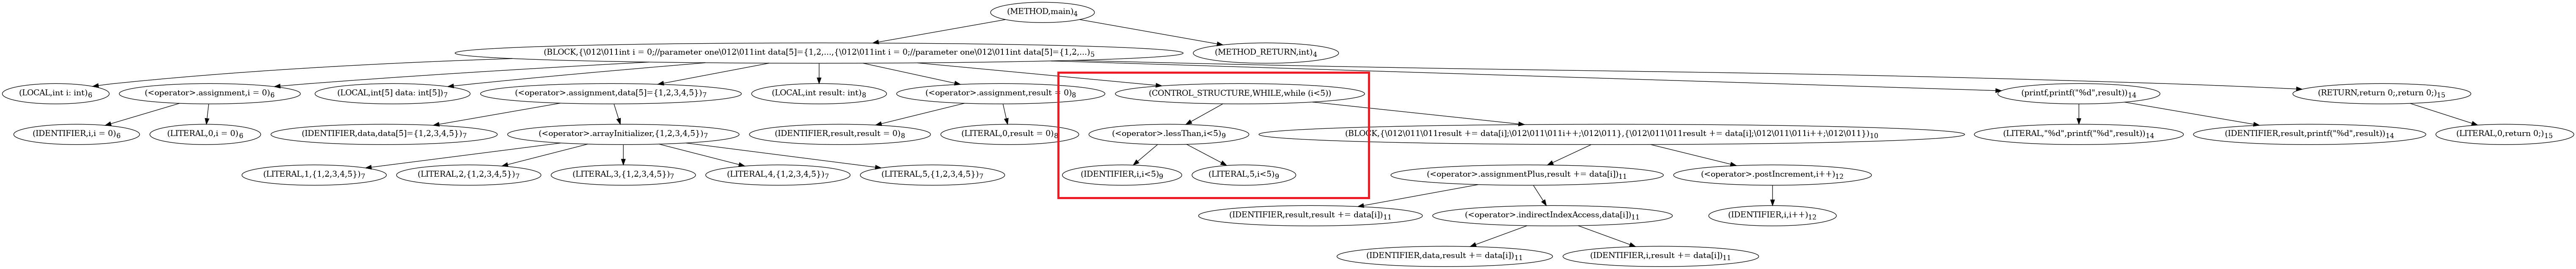
\includegraphics[width=0.3\textwidth]{figures/ast2}
      \label{fig:ast2} %引用标签
  }
  \subfigure[代码片段3对应的AST]{ %第三张子图
      \centering    %子图居中
      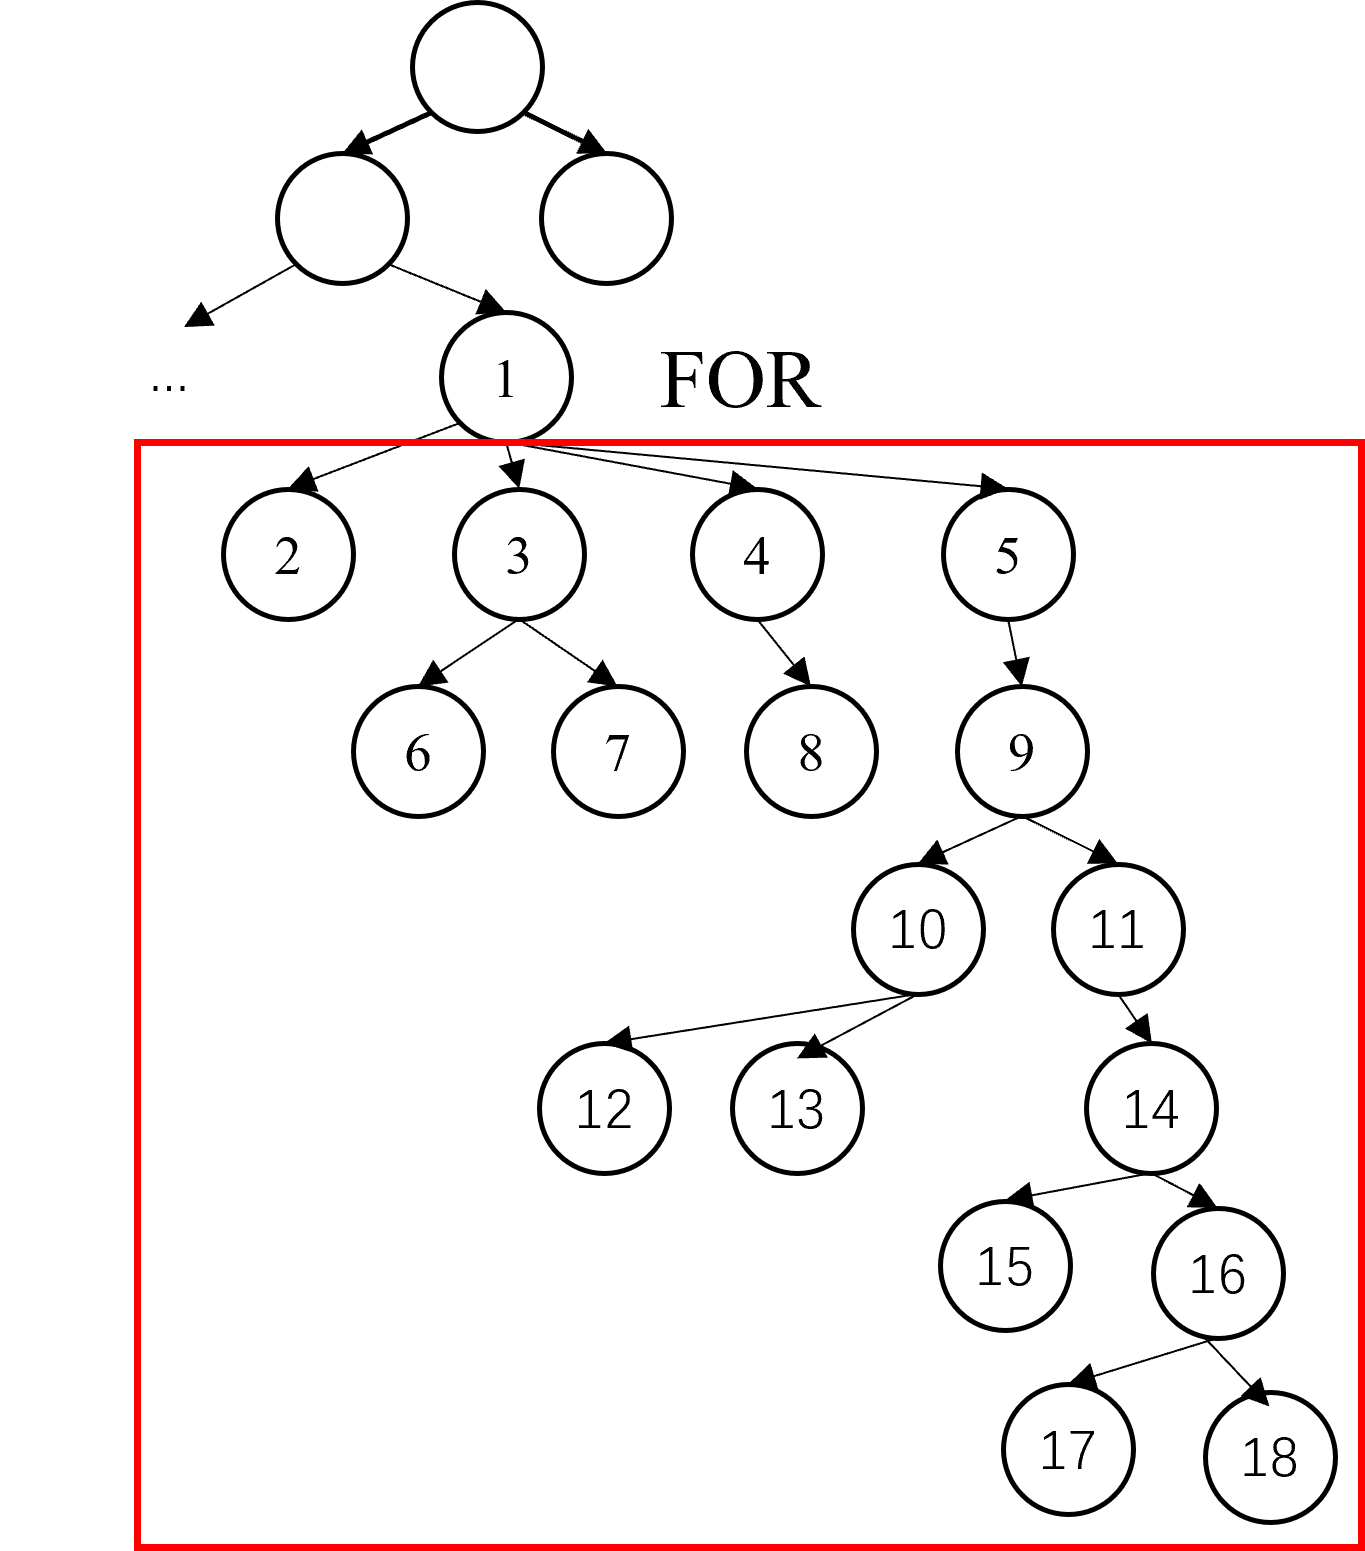
\includegraphics[width=0.3\textwidth]{figures/ast3}
      \label{fig:ast3} %引用标签
  }
  \caption{示例源代码对应的抽象语法树}    %大图名称
  \label{fig:astcode}    %图片引用标记
\end{figure}

接下来,本章提出的基于子树划分的抽象语法树表征学习方法的实现如图\ref{fig:ast}所示。该方法的输入是一对代码片段$C_{a},C_{b}$对应的抽象语法树,表示为$AST_{a},AST_{b}$,输出是$C_{a},C_{b}$对应的结构特征向量 $V_{a}^{AST},V_{b}^{AST}$,整体采用Siamese架构,两个子网络共享权值,从下到上,主要包括子树划分、子树表征、树表征三个阶段。

\begin{figure}[H]
  \centering
  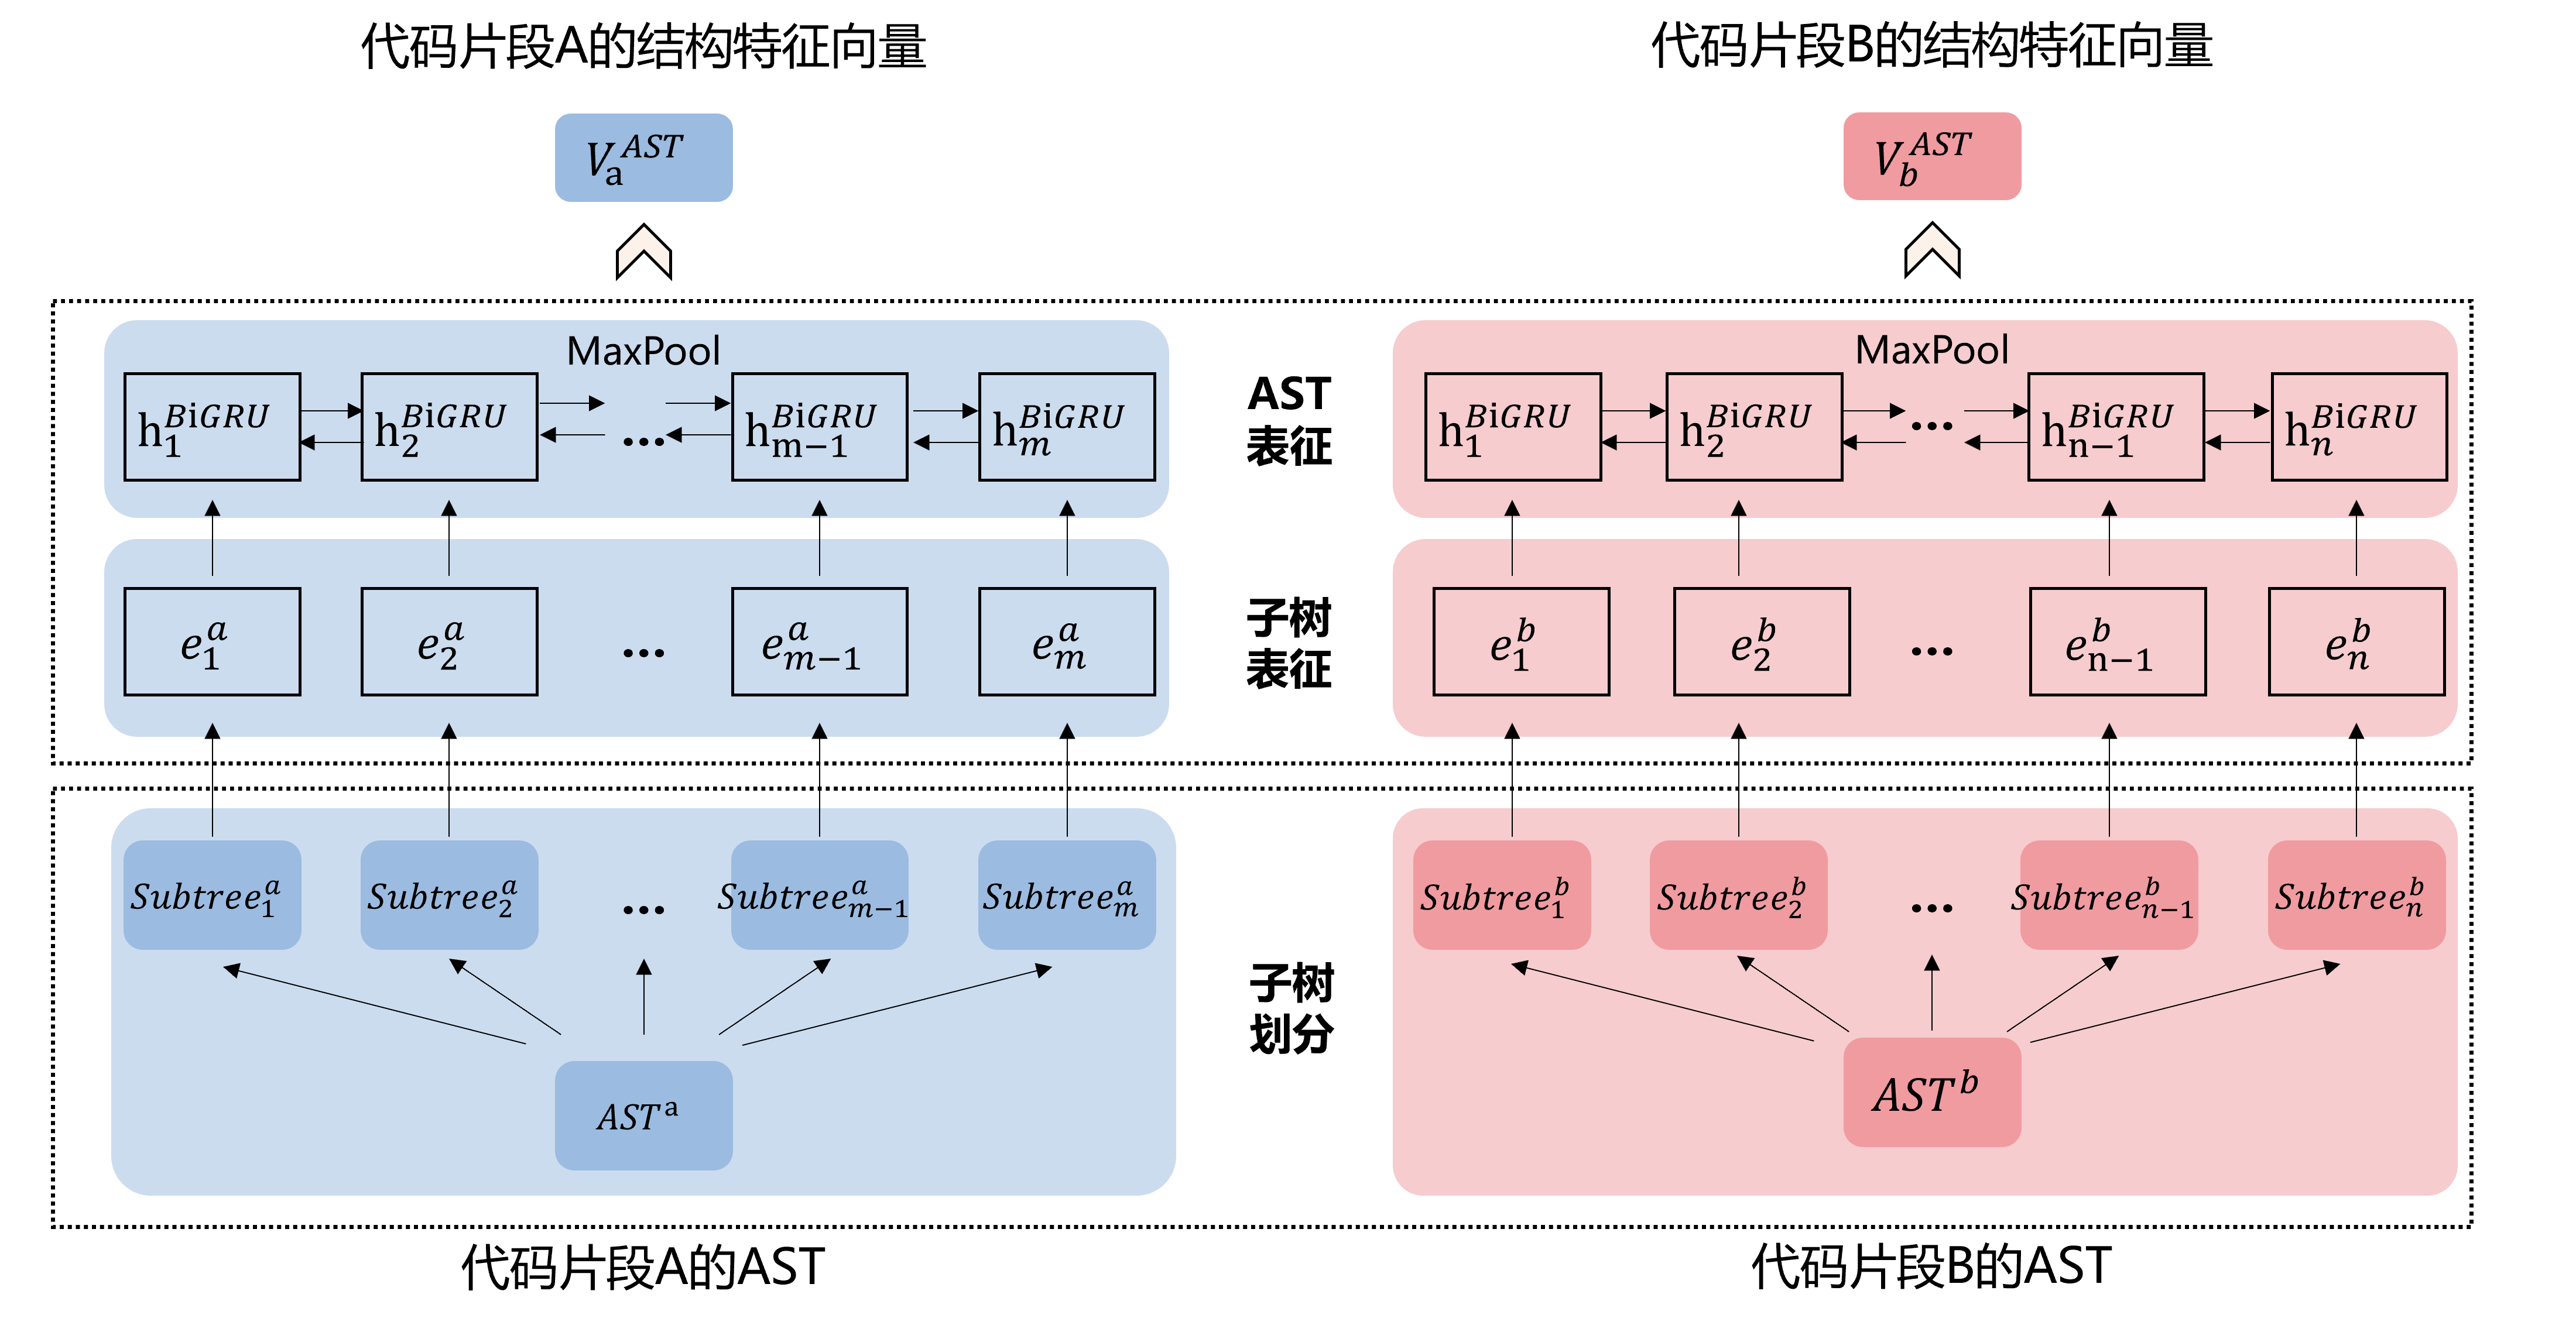
\includegraphics[width=0.8\textwidth]{figures/ast}
  \caption{基于子树划分的抽象语法树表征学习方法实现}\label{fig:ast}
\end{figure}

具体来说,在子树划分阶段,对于代码片段$C_{a}$,经过Joern代码分析工具生成得到抽象语法树$AST_{a}$,通过子树划分算法,可以得到子树序列,用$\left(SubTree_{1}^{a},SubTree_{2}^{a},\ldots,SubTree_{1}^{m}\right)$表示,$m$是子树序列的长度。其子树划分过程可以表示为公式\ref{e4.3}:

\begin{equation}\label{e4.3}
  \begin{split}
    \left(SubTree_{1}^{a},SubTree_{2}^{a},\ldots,SubTree_{m}^{a}\right) = split \left(AST_{a}\right)
  \end{split}
\end{equation}

经过子树划分后,代码片段$C_{a}$生成了子树序列$\left(SubTree_{1}^{a},SubTree_{2}^{a},\ldots,SubTree_{m}^{a}\right)$。使用同样的划分方法,可以得到代码片段$C_{b}$生成了子树序列$\left(SubTree_{1}^{b},SubTree_{2}^{b},\ldots,SubTree_{n}^{b}\right)$,$n$是代码片段$C_b$对应的子树序列长度。

在树表征阶段,首先将代码片段的子树序列作为输入,使用基于树的卷积神经网络模型进行编码,得到每个子树对应的语句向量$\left( e_{1}^{a},e_{2}^{a},\ldots,e_{m}^{a}\right)$。然后,使用双向门控循环单元(BiGRU)来模拟语句的自然性,通过最大池化层将BiGRU的隐藏状态采样到单个固定长度的向量$V_{a}^{AST}$中,作为最终的抽象语法树表示,即结构特征向量。具体的处理过程如公式\ref{e4.4}
\begin{equation}\label{e4.4}
  \begin{split}e
    h_{1}^{aBiGRU},h_{2}^{aBiGRU},\ldots,h_{n}^{aBiGRU} = BiGRU \left(e_{1}^{a},e_{2}^{a},\ldots,e_{m}^{a}\right) \\
    V_{a}^{AST} = MaxPool \left( h_{1}^{aBiGRU},h_{2}^{aBiGRU},\ldots,h_{n}^{aBiGRU} \right)
  \end{split}
\end{equation}

同样,可以使用相同的计算以子树序列$\left(SubTree_{1}^{b},SubTree_{2}^{b},\ldots,SubTree_{n}^{b}\right)$作为输入为代码片段$C_{b}$计算$V_{b}^{AST}$。


\section{实验验证}
\label{sec:ASTExperiment}

为了验证基于子树划分的抽象语法树表征学习方法的有效性,本文
\subsection{实验设计}
\label{subsec:ASTDesign}
和3.3.1 相同
\subsection{实验结果}
\label{subsec:TokenResult}
消融对比实验:体现AST子树划分的有效性

基于AST的Tree-LSTM

基于AST的+子树划分的Tree-LSTM

\begin{table}
  \centering
  \caption{抽象语法树子树划分实验结果} %{tab:category}
  \begin{tabular*}{0.9\textwidth}{@{\extracolsep{\fill}}cccc}
  \toprule
    对比			&P		&R		&F1 \\
  \midrule
    基于AST的Tree-LSTM			&0.xx	&0.xx		&0.xx \\
    基于AST的+子树划分的Tree-LSTM			&0.xx		&0.xx		&0.xx \\
  \bottomrule
  \end{tabular*}
\end{table}

\section{本章小结}
\label{sec:Summary4}
本章主要对RLCCD中基于子树划分的抽象语法树表征学习方法的设计与实现进行详细阐述。首先介绍了抽象语法树维度的研究动机,其次介绍了抽象语法树表征学习的方法设计,具体论述了其整体框架、预子树划分、树表征学习,接着开展实验验证,结果表明了此方法的有效性和模型的准确性。



